\documentclass[letterpaper, 10 pt, conference]{ieeeconf}

\IEEEoverridecommandlockouts                              % This command is only needed if 
   % you want to use the \thanks command

\overrideIEEEmargins                                      % Needed to meet printer requirements.

% See the \addtolength command later in the file to balance the column lengths
% on the last page of the document

% The following packages can be found on http:\\www.ctan.org
\usepackage{graphicx} % for pdf, bitmapped graphics files
%\usepackage{epsfig} % for postscript graphics files
%\usepackage{mathptmx} % assumes new font selection scheme installed
%\usepackage{times} % assumes new font selection scheme installed
\usepackage{amsmath} % assumes amsmath package installed
%\usepackage{amssymb}  % assumes amsmath package installed

\graphicspath{ {images/} }

\title{\LARGE \bf
Agent Coordination and Reward Shaping* \\
ROB538 - HW3
}


\author{Ammar Kothari$^{1}$
\thanks{*This work was supported by Oregon State University}% <-this % stops a space
\thanks{$^{1}$Department of Robotics, School of MIME, Oregon State University
        {\tt\small kothariA@oregonstate.edu}}%
}


\begin{document}



\maketitle
\thispagestyle{empty}
\pagestyle{empty}


%%%%%%%%%%%%%%%%%%%%%%%%%%%%%%%%%%%%%%%%%%%%%%%%%%%%%%%%%%%%%%%%%%%%%%%%%%%%%%%%
\begin{abstract}
\label{sec:abstract}
This article discusses the challenges in solving a classic congestion problem.  Different reward structures benefits and drawbacks are discussed.  Ultimately, the difference reward with respect to a counterfactual performs best.  

\end{abstract}


%%%%%%%%%%%%%%%%%%%%%%%%%%%%%%%%%%%%%%%%%%%%%%%%%%%%%%%%%%%%%%%%%%%%%%%%%%%%%%%%
\section{INTRODUCTION}
\label{sec:intro}

Congestion is an ever growing problem in today's world.  Shop floor production, street traffic, and energy plant efficiency are common areas that continue to experience increased difficulties due to congestion.  By finding a way for many distributed sites to collaborate to solve a problem without centralized control could improve our daily lives.  All of these issues share the common constraint that there are too many things or people that need to use the limited resources.


\section{BACKGROUND}
\label{sec:background}
El Faro's bar problem is a classic congestion problem.  An ideal attendance is desired throughout the week, but too many agents are present to achieve optimal performance through even distribution.  Additionally, each agent's actions are part of the environment further complicating learning in the system.  El Faro's approach to the system is that any deductive reasoning approach would likely be insufficient as the system grows.  He shows that an inductive approach would be very capable and efficient at solving this problem.

In this simulation, the reward is given as:

\begin{equation}
    G(z) = \displaystyle\sum_{k=1}^{K} x_{k}(z)e^{\frac{-x_{k}(z)}{b}}
\end{equation}
\begin{itemize}
    \item G is the system reward for the week
    \item $x_{k}(z)$ is the attendance on a given night
    \item K is the number of nights in a week that the bar is open
    \item b is the optimal attendance for the bar.  This is the same every night.
\end{itemize}

\section{Method}
\label{sec:method}
Each agent has a set of action-values corresponding to each night.  These values are initialized to a large value ($>20$) to ensure that the agent explores other nights.  Another promoter for exploration is to allow agents to choose their actions using an $\epsilon$-greedy method.  In the simulation, $\epsilon$ is set to 5\% and decreases by 1\% from the previous week.  Early exploration helps an agent find a good solution.  Exploration later on in the process provides little value.  

After an agent decides on an action, they receive a reward.  This is incorporated into their action-value set by:
\begin{equation}
    K_i^{new} = K_i^{old} + \alpha*(r_{c,t} - K_i^{old})
\end{equation}
\begin{itemize}
    \item $K_i$ is the value for an action.
    \item $\alpha$ is the learning rate.  In the simulation, it was set to 0.01.
    \item $r_{c,t}$ is the reward for a choice at a certain time step.
\end{itemize}

In this article, a proven system for iteratively solving this problem is analyzed.  The counter-factual comparison is effective in achieving and maintaining equilibrium in this system.

\section{Analyzed Solutions}
\label{sec:proposed solutions}
\subsection{Local Reward}
A local reward is a reward that is applicable to an agent and can be determined based on observations the agent can make.  One sensible local reward is to simply reward each agent with the reward based on the night they attended the bar.  
\begin{equation}
    L(z) = x_{k_i}(z)e^{\frac{-x_{k_i}(z)}{b}}
\end{equation}

\begin{itemize}
    \item $x_{k_i}(z)$ is the night that the agent choose to attend.
\end{itemize}

For example, an agent who attends on Tuesday night will receive the part of the global reward that was contributed by Tuesday night.

This reward has low learnability.  The large number of other agents creates a lot of noise in the system.  The agent receives a reward for an action, but may not receive a similar reward the next time they take that action.  An agent cannot discern a good action from good circumstance.  This reward is also not aligned with the system goal.  The agent will attempt to maximize their own reward by attending a night that has the closest to optimal attendance.  However, in order to maximize the system goal, an agent may need to sacrifice a personal reward for the greater system reward.  An agent may move from one night to another night such that the local reward increases, but the system reward decreases.  A better solution would align the agents actions with what is good for the system.

A different reward that could be useful is a local difference reward.  One method of implementing this is to compare the reward if an agent attended to the reward if an agent had stayed at home.  
\begin{equation}
    D^{local}(z) = L^{current}(z) - L^{-i}
\end{equation}
\begin{itemize}
    \item $L^{current}(z)$ is the reward with the agents actions
    \item $L^{-i}$ is the reward if the agent had stayed at home (i.e. not existed)
\end{itemize}

An agent can gauge their impact on the success of the night by determining how much more of less value was added by attending.  For similar reasons as the previous reward structure, this reward is also not very learnable.  The agent will still have a hard time differentiating a good action from a fortunate circumstance.  Although in this case, the noise of the other agents attending that night is removed.  This policy is also not aligned with the system reward.  The agent will still move towards situations that provide the highest local reward. Again, agent local reward will never be sacrificed to promote system reward.


 Benefits of both of these approaches is that all the information that an agent needs to determine the reward is locally available.  Although, they are required to know the equation for determining reward, all other information should be available once at the bar.

\subsection{Counterfactual Difference Reward}
An alternate reward that could be used is the counterfactual reward.  An extension of the previous difference reward is to examine global system reward with the agent and with a null counterfactual agent (i.e. agent does not exist).  However, upon closer inspection, the global reward without replacement and the local reward without replacement are identical.  Since the change is only being done to a single night, only one value in the global reward changes.
\begin{equation}
\begin{aligned}
    D^{global}_{no replace} &= G^{current} - G^{-i} \\
    &= L^{current}_0 + ... + L^{current}_k + ... + L^{current}_n \\
     &- (L^{current}_0 + ... + L^{-i}_{k} + ... + L^{current}_n) \\
    &= L^{current}_k - L^{-i}_k
\end{aligned}
\end{equation}

This solution will suffer from the same drawbacks as previously discussed.

A slightly altered approach that could be successful is to define the counterfactual as an agent that attends on another night.  Many options exist for how to add the counterfactual back to the system.  In this article, adding the agent back to a standard night is examined.
\begin{equation}
\begin{align}
    D^{global}_{replace} &= G^{current} - G^{-i}_{+i} \\
    &= L^{current}_{k-night} + L^{current}_{cf-night} - L^{-i}_{k-night} - L^{+i}_{cf-night}
\end{align}
\end{equation}

\begin{itemize}
    \item $G^{-i}_{+i}$ is the system reward if the agent had attended an alternate night
    \item $k-night$ is the night that the agent attended
    \item $cf-night$ is the "standard" night
    \item $L^{+i}$ is the local reward with one additional person
\end{itemize}
This reward is comparing the effect that the agent has by attending a given night over attending a standard night.  This reward is more learnable than the previous rewards because some of the noise caused by the other agents is removed.  It is also aligned with the system reward.  An agent can understand that sacrificing local reward can benefit the system.  



\section{RESULTS}
\label{sec:results}
In this section, the results for simulating the bar problem with different rewards and different simulation parameters are shared.  The simulation is allowed to run up to 100,000 weeks, but all steady state behavior is achieved in the first 20,000 weeks.  For each reward system, 10 trials were run to also examine statistical occurrence of solutions.

For the distribution of attendance, the final 10 weeks of the trial are averaged.  This clearly captures any variation that is still occurring.  For the histograms, the agent attendance is not shown below zero since negative attendance does not have a realistic interpretation in this situation.  The attendance for each trial is also sorted from minimum to maximum and averaged in those groups.  Given the random nature of the system, it is possible for the same starting condition to converge to solutions that inhabit different days of the week, but are functionally equivalent.  Sorting clarifies trends independent of night.

The reward in the scatter plots is an average reward for the system in that time period.

\subsection{Scenario 1}
In scenario 1, 30 agents are trying to optimally attend 7 nights at a bar with an ideal attendance of 4 people.  In this scenario, 28 agents would be able to attend the bar with optimal attendance.  There is a slight congestion.
\begin{figure}
    \centering
    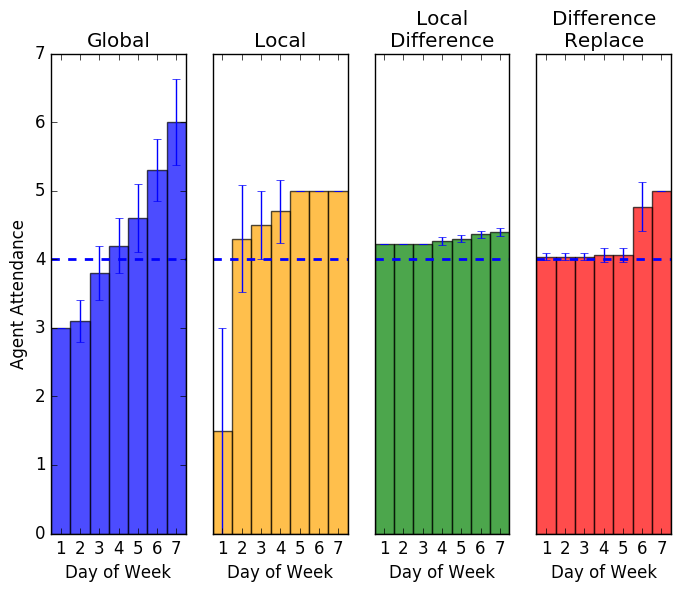
\includegraphics[width=230pt]{Histograms0.png}
    \caption{Histogram of attendance for different reward structures when N=30,k=7,b=4}
    \label{fig:Scenario1_hist}
\end{figure}

\begin{figure}
    \centering
    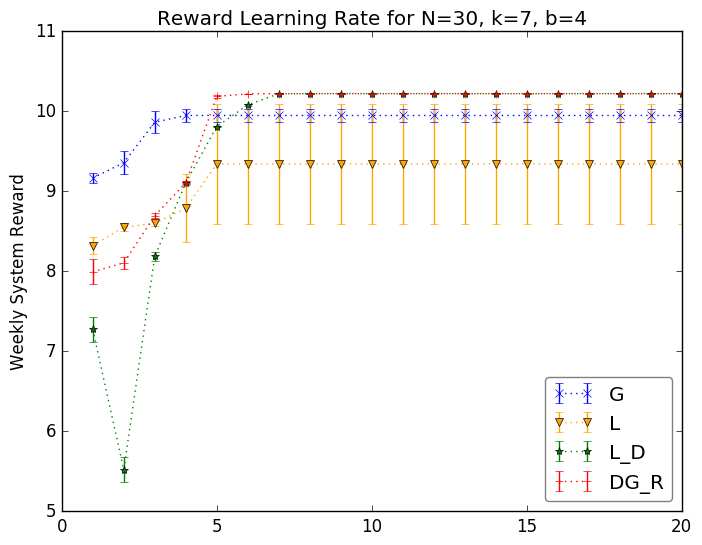
\includegraphics[width=230pt]{Scatter0.png}
    \caption{Plot of average reward per week for different reward structures when N=30,k=7,b=4}
    \label{fig:scenario1_scatter}
\end{figure}



In scenario 2, 40 agents are trying to optimally attend 5 nights at a bar with an ideal attendance of 5 people.  In this scenario, 25 agents would be able to attend the bar with optimal attendance.  The congestion here is worse here than in the previous scenario.
\begin{figure}
    \centering
    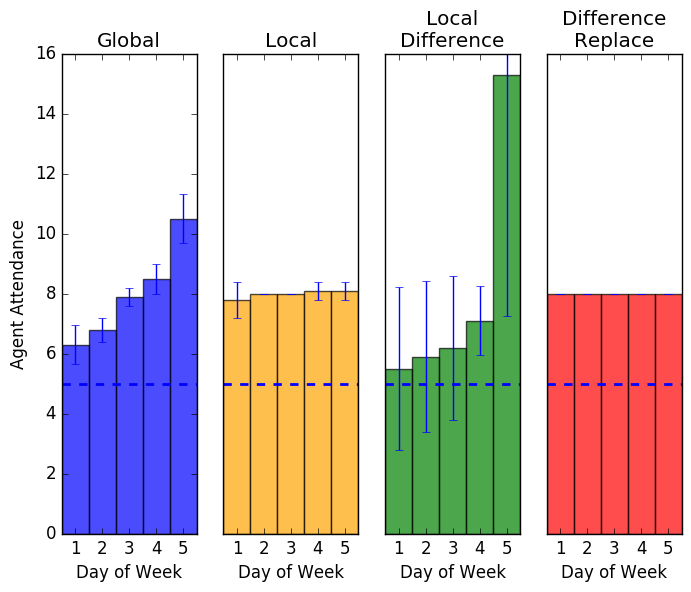
\includegraphics[width=230pt]{Histograms1.png}
    \caption{Histogram of attendance for different reward structures when N=40,k=5,b=5}
    \label{fig:Scenario2_hist}
\end{figure}

\begin{figure}
    \centering
    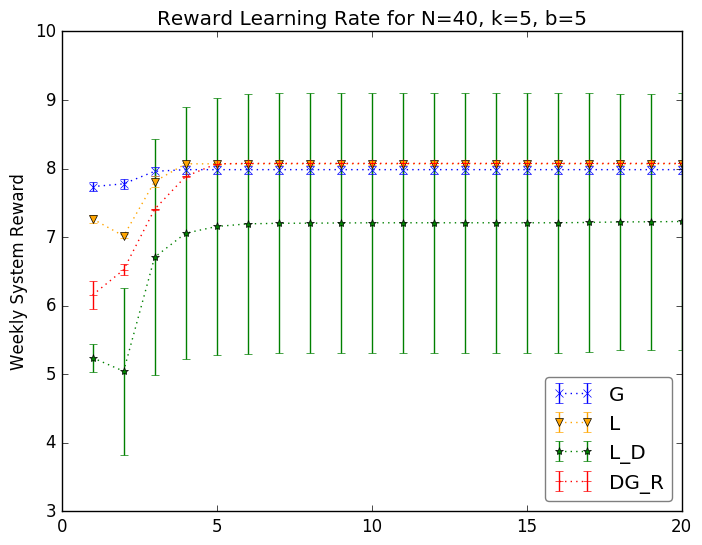
\includegraphics[width=230pt]{Scatter1.png}
    \caption{Plot of average reward per week for different reward structures when N=40,k=5,b=5}
    \label{fig:scenario2_scatter}
\end{figure}

Scenario 3 is the same as scenario 2 except that there are now 100 agents.  The congestion here is the worst of all scenarios.
\begin{figure}
    \centering
    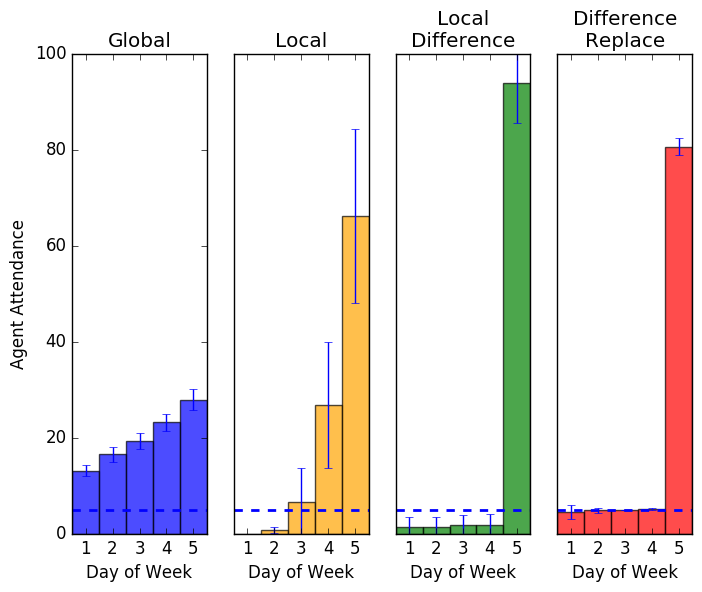
\includegraphics[width=230pt]{Histograms2.png}
    \caption{Histogram of attendance for different reward structures when N=100,k=5,b=5}
    \label{fig:Scenario3_hist}
\end{figure}

\begin{figure}
    \centering
    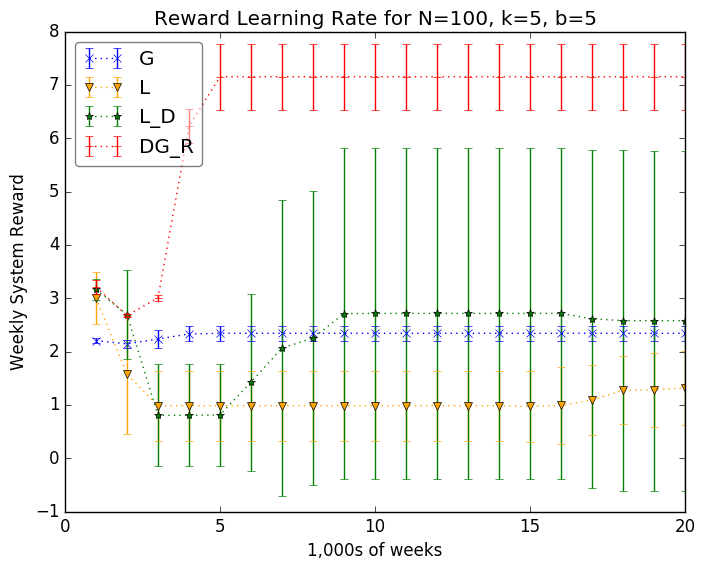
\includegraphics[width=230pt]{Scatter2.png}
    \caption{Plot of average reward per week for different reward structures when N=100,k=5,b=5}
    \label{fig:scenario3_scatter}
\end{figure}

\section{ANALYSIS}
\label{sec:analysis}
\subsection{Global Reward}
In both scenario 1 and 2, the global reward performs almost as well as the other two rewards.  It even converges faster to its final value than any other method.  The ability of this reward structure to quickly achieve a high system reward is note worthy.  There is some fluctuation in attendance, but it is not more than other policies.  Since congestion is low, the variation which may be centered around even distribution produces a high system reward.  The global reward may be the preferred reward structure in a situation where convergence time is more important than a slightly higher steady state value.  This could be applicable in slight and moderate congestion problems.

The global reward does not fair so well in the heavily congested third scenario.  The global reward is unable to cause the agents to improve upon their initial reward values.  One explanation is that the amount of noise produced by having so many agents may make it very difficult for the agents to learn.  An alternate description of the agents movements is that they are again fluctuating around an even distribution.  However, in this scenario, there is not a high system reward for being close to evenly distributed.  The global reward is not suitable for situations when the resources are severely limited.

\subsection{Local Reward}
The local reward causes the agents act independent of the overall reward.  The agent is encouraged less to return for nights without optimal attendance. However, given the reward structure, an agent is punished more for attending a night with one fewer person than for attending a night with one more person.  This likely causes the agents to move around a lot more in scenario 1 instead of settling on a solution.  The agents are tending towards slightly higher attendance, which creates lower attendance on other nights.  This creates imbalance and the system cannot settle.  Along the same lines, it is possible for a night to become too unfavorable.  As fewer agents attend, the reward drops and the reward received for attending a night with fewer people is smaller than attending a night with too many people.  A night with three less agents is much more unfavorable than a night with three too many agents.  The local reward can enter a devaluation spiral.

Comparatively, the variation in scenario 2 is much less because the reward difference between one too many agents and one fewer agents is smaller than in scenario 1.  The local reward is able to achieve almost the maximum reward.  The local reward is a good solution here.  It also has the benefit of being entirely observable by the agent.  

In scenario 3, the agents are not able to settle on a solution.  Significant movement continues to occur without any improvement in system reward.  It is interesting that the agents do not settle on an even distribution.  Convergence may be occurring so slowly due the noisiness of the signal that it could not even be extracted from the data despite 100,000 weeks.

The local reward does not produce the desired behavior in most situations, but explaining the agents actions is not easy.

\subsection{Difference Rewards}
\subsubsection{Local}
The local difference reward is slightly better than the local reward in low and high levels of congestion.  The difference reward gives a stronger signal of what is a bad choice.  The agent knows whether he is pushing the attendance in the right direction.  The result in scenario one is that the agent who is the 5th person at the bar, continues to move around and find a better spot.  She attempts each night only to find it would be better without that agent.  This can be seen clearly in figure \ref{fig:Scenario1_hist}.  The local difference reward achieves the maximum reward in scenario 1.  This is an improvement over the local reward with the same amount of information available.

The local difference action in scenario 2 and 3 seems incomprehensible.  The agents appear to be piling on to one day, but maintain a huge amount of movement.  In situations where a lot of variation is not good, the local difference award does not do as well as the local reward.  In scenario 3, a higher reward is achieved by being far from evenly distributed.  Local difference can stumble upon this solution, but the local reward is unlikely to.


\subsubsection{Global}
Finally, the global solution appears to perform the best.  It consistently achieves the highest reward with little variation.  Additionally, it is the only one capable of handling extreme congestion as in scenario 3.  In scenario 1 and 2, convergence takes longer than other reward strategies.  The longer convergence is because the counterfactual night does not become beneficial until enough agents attend.  Initially, when there is high variation, the signal from the "standard" night is very noisy.  As the system settles, this signal is more effective at aligning the agents actions with the system reward.  Overall though, the best performance is achieved by the global difference reward.  As a drawback, the global difference reward requires the agent to have non-local information.  Each agent needs to know the attendance on the "standard" night as well as the attendance on the night they attended the bar.  In comparison to the local and global reward, the difference rewards require twice as many calls to G.  In this case, that is not meaningful, but in other applications, this could require significantly more processing power.

\section{FUTURE WORK}
\label{sec:futurework}
There are many applications where a multiagent approach to congestion problems can improve the system performance in the real world.  Given the prevalence of these situations, many investigations can be done to see if an optimal solution is implemented and what reward shaping needs to be done in order to achieve optimal performance.

Further investigation of the devaluation spiral would be interesting.  It may shed light on how a system with local rewards can perform far worse than initially anticipated.

Instead of using the reward function, allowing each agent to approximate the reward function internally would create an interesting dynamic.  They would effectively be predicting the actions of other agents in the system by attempting to predict the reward structure.

\section{CONCLUSION}
\label{sec:conclusion}
Congestion problems are not going away.  Resource constraint is a growing problem.  By investigating toy problems like the bar problem, we can develop insight into how to effectively solve real congestion problems.  Local rewards can provide some success, but do not work in all situations.  A local difference reward is even more unpredictable, but can, in certain cases, improve performance.  A global reward has too much noise to be effective in large systems, but can help in small systems.  The difference global reward is the most effective.  It has the best performance at multiple congestion levels.



%\bibliographystyle{IEEEtran}
%\bibliography{IEEEabrv,IEEEexample}

\end{document}
